% ******************************* Thesis Appendix E ********************************
\chapter{} 
\label{app:NoWindMaps}

\graphicspath{{Appendix5/Figs/}}

\renewcommand{\thefigure}{E\arabic{figure}}

\setcounter{figure}{0}

The following 4 figures are the results of the testing scenarios attempting to fly Dubins path turns in a zero wind condition. The four configurations are:

\begin{enumerate}
	\item 65\degree  maximum roll angle, airspeed of 20 metres per second
	\item 65\degree  maximum roll angle, airspeed of 10 metres per second
	\item 32.5\degree  maximum roll angle, airspeed of 20 metres per second
	\item 32.5\degree  maximum roll angle, airspeed of 10 metres per second
\end{enumerate}

The figures appear in the order the configurations are listed here.


\begin{figure}[htbp!] 
\centering    
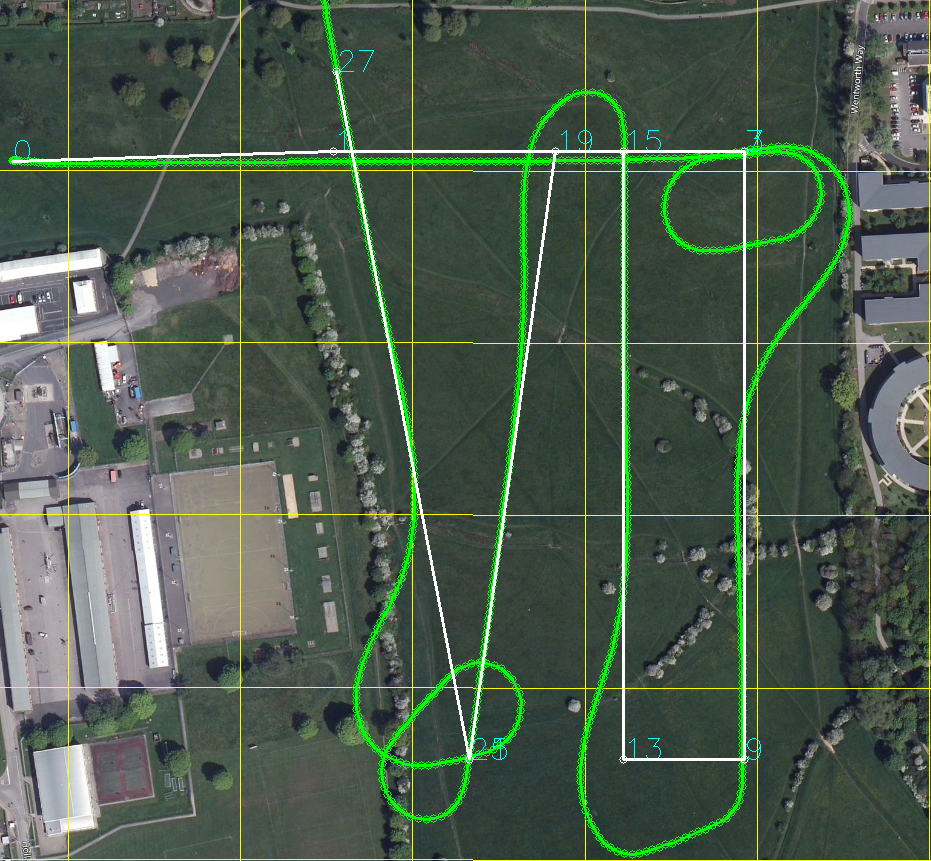
\includegraphics[width=\textwidth]{65_20_NoWind}
\caption{A trace of the path the UAV flew when commanded to fly in the absence of wind, with a 65\degree  maximum roll angle, and at an airsped of 20 metres per second}
\end{figure}

\begin{figure}[htbp!] 
\centering    
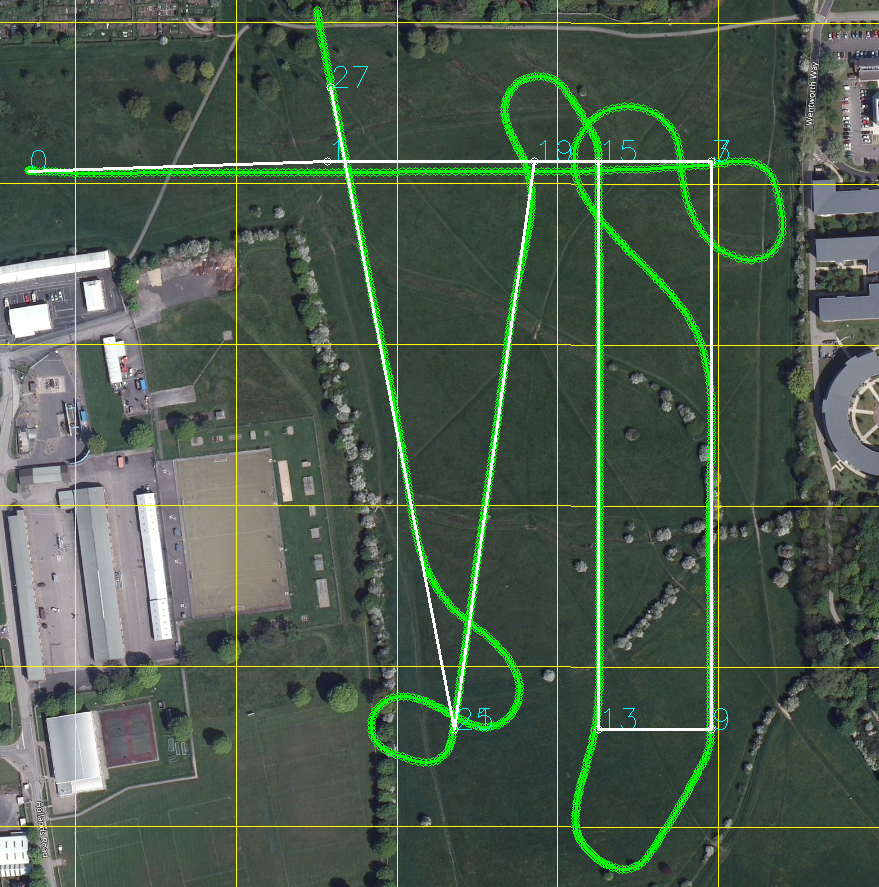
\includegraphics[width=\textwidth]{65_10_NoWind}
\caption{A trace of the path the UAV flew when commanded to fly in the absence of wind, with a 65\degree  maximum roll angle, and at an airsped of 10 metres per second}
\end{figure}

\begin{figure}[htbp!] 
\centering    
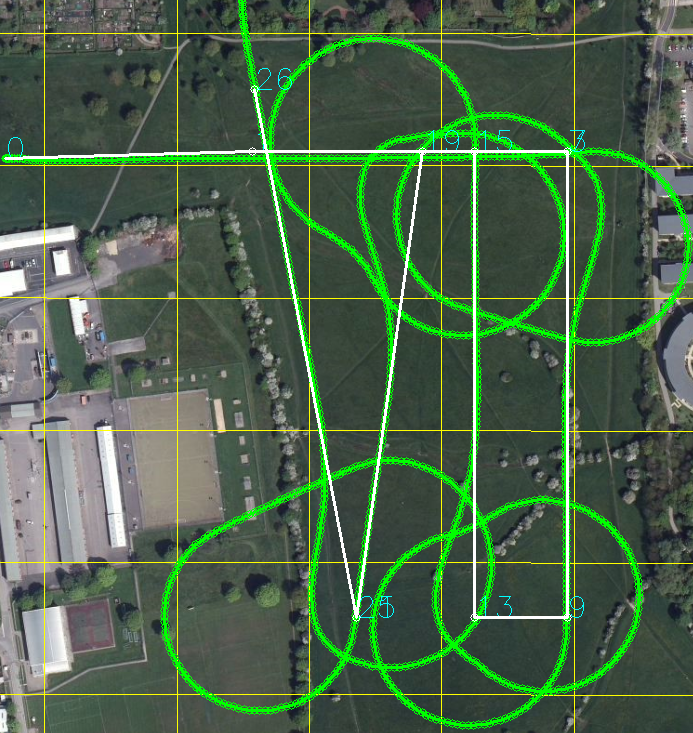
\includegraphics[width=\textwidth]{32_20_NoWind}
\caption{A trace of the path the UAV flew when commanded to fly in the absence of wind, with a 32.5\degree  maximum roll angle, and at an airsped of 20 metres per second}
\end{figure}

\begin{figure}[htbp!] 
\centering    
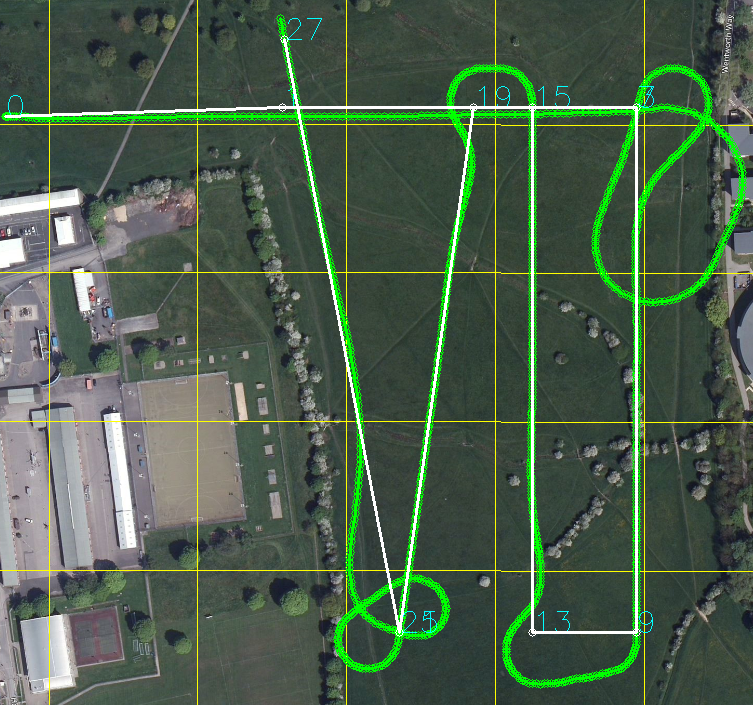
\includegraphics[width=\textwidth]{32_10_NoWind}
\caption{A trace of the path the UAV flew when commanded to fly in the absence of wind, with a 32.5\degree  maximum roll angle, and at an airsped of 10 metres per second}
\end{figure}